\chapter{Выполнение лабораторной работы №7}
\label{ch:lab7}

\section{Выбор набора данных}

Для выполнения лабораторной работы используется набор данных \textbf{Abalone}, который содержит следующие характеристики:

\begin{itemize}
    \item Количество записей: 4177
    \item Количество признаков: 8
    \item Категориальный признак: \texttt{Sex} (M --- мужской, F --- женский, I --- детеныш)
    \item Числовые признаки: Length, Diameter, Height, Whole weight, Shucked weight, Viscera weight, Shell weight
    \item Целевая переменная: \texttt{Rings} (количество колец на раковине)
\end{itemize}

\section{Теоретическое обоснование}

При решении задач многомерной регрессии исследователю необходимо решить ряд подзадач:

\begin{enumerate}
    \item Определить коррелированность признаков.
    \item Определить, какие признаки существенны при построении модели регрессии.
\end{enumerate}

Проблема определения значимых признаков связана с проблемой снижения размерности. Важное значение при многомерной регрессии приобретает обработка категориальных признаков. Часто необходимо заменить категориальный признак на набор фиктивных переменных (One-Hot Encoding).

\subsection{Стратегии выбора значимых переменных}

К проблеме выбора значимых переменных существует несколько подходов:

\begin{itemize}
    \item \textbf{All-in} — включение всех признаков в модель.
    \item \textbf{Backward Elimination} — удаление признаков по одному на основе их значимости до достижения ситуации, когда останутся только значимые признаки.
    \item \textbf{Forward Selection} — добавление наиболее значимых признаков.
    \item \textbf{Bidirectional Elimination} — комбинация стратегий 2 и 3.
\end{itemize}

\section{Ход выполнения работы}

\subsection{Шаг 1: Загрузка и первичный анализ данных}

\begin{lstlisting}[language=Python, caption=Загрузка и анализ данных]
import numpy as np
import matplotlib.pyplot as plt
import pandas as pd
import seaborn as sns
from sklearn.model_selection import train_test_split
from sklearn.linear_model import LinearRegression
from sklearn.metrics import mean_squared_error, r2_score
from sklearn.preprocessing import StandardScaler
import statsmodels.api as sm

df = pd.read_csv('abalone.csv')
print(f"Размер набора данных: {df.shape}")
print("\nПервые 5 строк:")
print(df.head())

print("\nИнформация о данных:")
print(df.info())
\end{lstlisting}

Результат:

\begin{verbatim}
Размер набора данных: (4177, 9)

Первые 5 строк:
  Sex  Length  Diameter  Height  Whole weight  Shucked weight  Viscera weight  Shell weight  Rings
0   M   0.455     0.365   0.095         0.514          0.2245           0.101         0.150     15
1   M   0.350     0.265   0.090         0.2255         0.0995          0.0485        0.070      7
2   F   0.530     0.420   0.135         0.677          0.2565          0.1415        0.210      9
3   M   0.440     0.365   0.125         0.516          0.2155          0.1140        0.155     10
4   I   0.330     0.255   0.080         0.205          0.0895          0.0395        0.055      7
\end{verbatim}

\subsection{Шаг 2: Анализ корреляции признаков}

\begin{lstlisting}[language=Python, caption=Корреляционный анализ]
numeric_cols = df.select_dtypes(include=[np.number]).columns
correlation_matrix = df[numeric_cols].corr()

plt.figure(figsize=(12, 10))
sns.heatmap(correlation_matrix, annot=True, cmap='coolwarm', center=0,
            square=True, linewidths=1, fmt='.2f')
plt.title('Корреляционная матрица признаков')
plt.tight_layout()
plt.savefig('lab7_correlation_matrix.png', dpi=150)

print("\nКорреляция признаков с целевой переменной Rings:")
correlations = df[numeric_cols].corr()['Rings'].sort_values(ascending=False)
for feat, corr in correlations.items():
    print(f"  {feat}: {corr:.4f}")
\end{lstlisting}

Результат:

\begin{verbatim}
Корреляция признаков с целевой переменной Rings:
  Rings: 1.0000
  Shell weight: 0.6275
  Diameter: 0.5747
  Length: 0.5567
  Whole weight: 0.5408
  Viscera weight: 0.5038
  Shucked weight: 0.4209
  Height: 0.3894
\end{verbatim}

\begin{figure}[h]
\centering
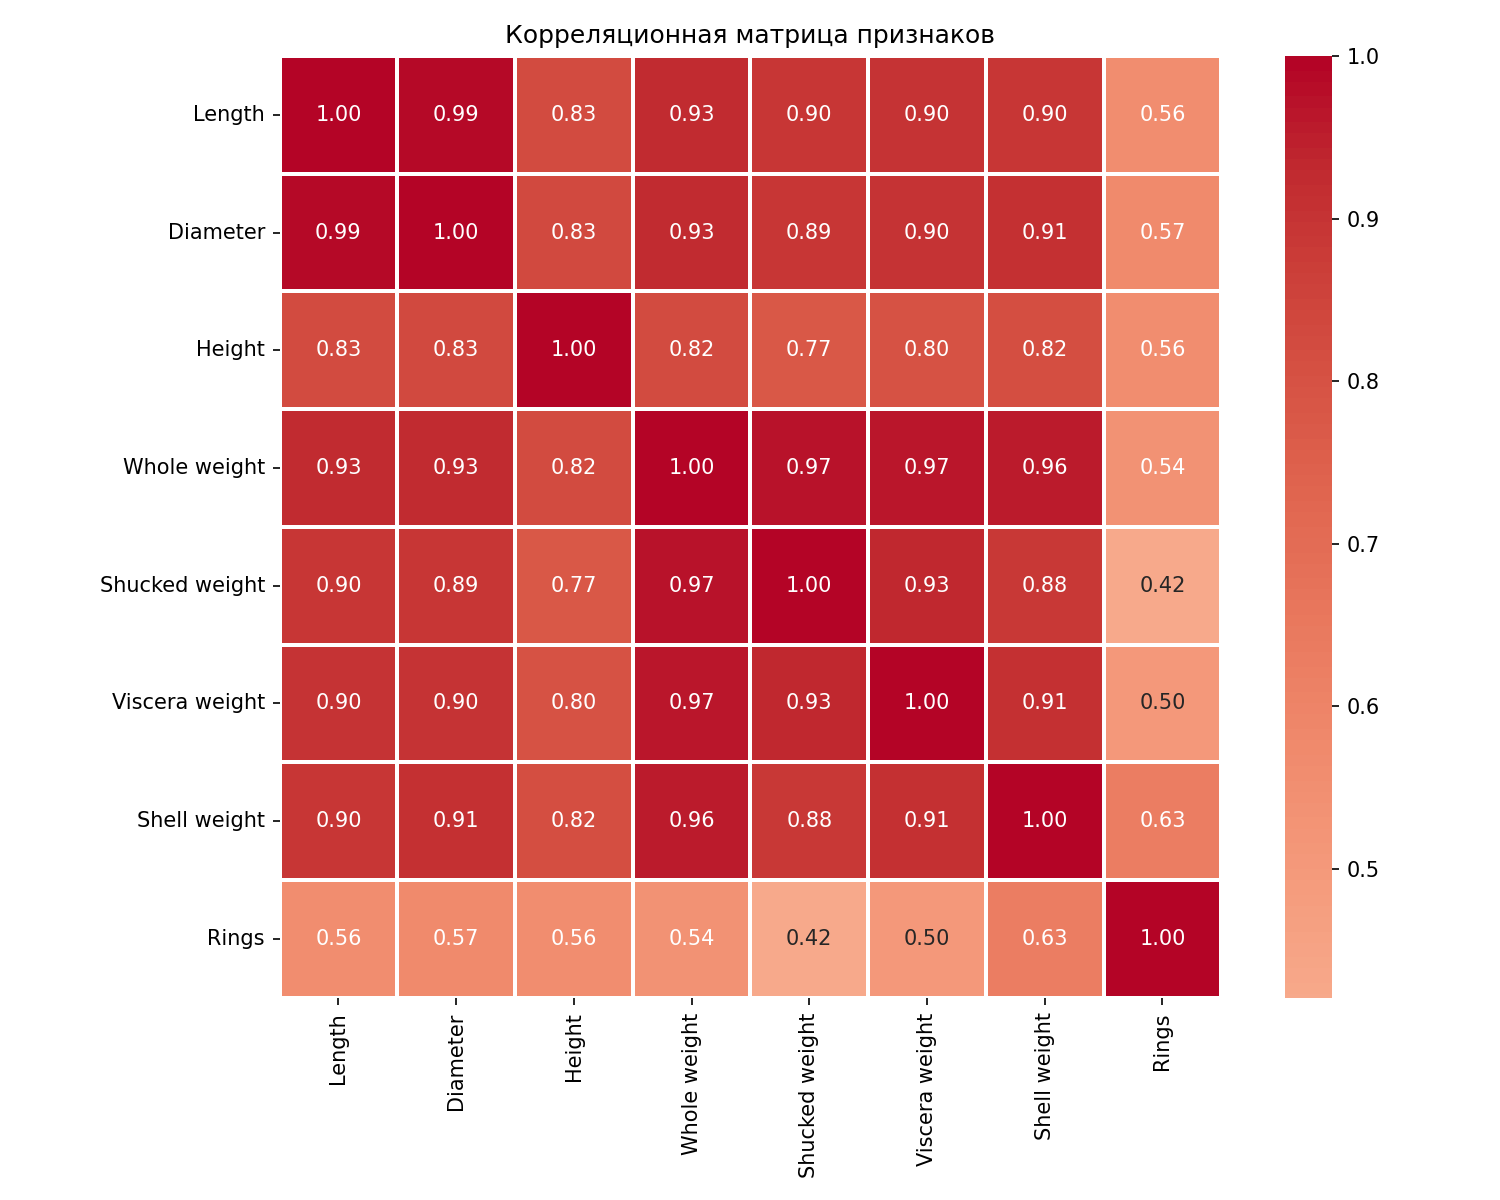
\includegraphics[width=0.8\textwidth]{lab7_correlation_matrix.png}
\caption{Корреляционная матрица числовых признаков}
\label{fig:lab7_correlation}
\end{figure}

Анализ корреляционной матрицы показывает сильную положительную корреляцию между всеми весовыми признаками, а также ожидаемую корреляцию между длиной и диаметром. Целевая переменная Rings имеет наибольшую корреляцию с признаком Shell weight.

\subsection{Шаг 3: Обработка категориальных данных}

\begin{lstlisting}[language=Python, caption=One-Hot Encoding]
X = df.drop('Rings', axis=1)
y = df['Rings']

categorical_features = X.select_dtypes(include=['object']).columns.tolist()
print(f"Категориальные признаки: {categorical_features}")

X_encoded = pd.get_dummies(X, columns=categorical_features, drop_first=True)
print(f"\nРазмер данных после One-Hot Encoding: {X_encoded.shape}")
print(f"Новые признаки: {[col for col in X_encoded.columns if 'Sex' in col]}")
\end{lstlisting}

Результат:

\begin{verbatim}
Категориальные признаки: ['Sex']

Размер данных после One-Hot Encoding: (4177, 10)
Новые признаки: ['Sex_I', 'Sex_M']
\end{verbatim}

\subsection{Шаг 4: Разделение на обучающую и тестовую выборки}

\begin{lstlisting}[language=Python, caption=Разделение данных]
X_train, X_test, y_train, y_test = train_test_split(
    X_encoded, y, test_size=0.2, random_state=42
)
print(f"Размер обучающей выборки: {X_train.shape}")
print(f"Размер тестовой выборки: {X_test.shape}")
\end{lstlisting}

Результат:

\begin{verbatim}
Размер обучающей выборки: (3341, 9)
Размер тестовой выборки: (836, 9)
\end{verbatim}

\subsection{Шаг 5: Модель со всеми признаками (All-in)}

\begin{lstlisting}[language=Python, caption=Обучение модели All-in]
regressor_all = LinearRegression()
regressor_all.fit(X_train, y_train)
y_pred_train_all = regressor_all.predict(X_train)
y_pred_test_all = regressor_all.predict(X_test)

train_mse_all = mean_squared_error(y_train, y_pred_train_all)
test_mse_all = mean_squared_error(y_test, y_pred_test_all)
train_r2_all = r2_score(y_train, y_pred_train_all)
test_r2_all = r2_score(y_test, y_pred_test_all)

print("\n=== Модель со всеми признаками (All-in) ===")
print(f"MSE на обучающей выборке: {train_mse_all:.4f}")
print(f"MSE на тестовой выборке: {test_mse_all:.4f}")
print(f"R² на обучающей выборке: {train_r2_all:.4f}")
print(f"R² на тестовой выборке: {test_r2_all:.4f}")
\end{lstlisting}

Результат:

\begin{verbatim}
=== Модель со всеми признаками (All-in) ===
MSE на обучающей выборке: 4.9795
MSE на тестовой выборке: 5.2505
R² на обучающей выборке: 0.5292
R² на тестовой выборке: 0.5155
\end{verbatim}

\subsection{Шаг 6: Backward Elimination с использованием p-значений}

\begin{lstlisting}[language=Python, caption=Анализ p-значений]
X_train_with_const = sm.add_constant(X_train)
model = sm.OLS(y_train, X_train_with_const).fit()
print("\n=== Статистика модели (p-значения) ===")
p_values = model.pvalues
for var, p_val in p_values.items():
    print(f"  {var}: p = {p_val:.6f}")
print(f"\nR² скорректированный: {model.rsquared_adj:.4f}")

significant_vars = p_values[p_values < 0.05].index.tolist()
if 'const' in significant_vars:
    significant_vars.remove('const')
print(f"\nЗначимые признаки (p < 0.05): {significant_vars}")
\end{lstlisting}

Результат:

\begin{verbatim}
=== Статистика модели (p-значения) ===
  const: p = 0.000000
  Length: p = 0.002354
  Diameter: p = 0.000382
  Height: p = 0.000000
  Whole weight: p = 0.000000
  Shucked weight: p = 0.000000
  Viscera weight: p = 0.000000
  Shell weight: p = 0.000000
  Sex_I: p = 0.000014
  Sex_M: p = 0.000000

R² скорректированный: 0.5283

Значимые признаки (p < 0.05): ['Length', 'Diameter', 'Height', 'Whole weight', 
'Shucked weight', 'Viscera weight', 'Shell weight', 'Sex_I', 'Sex_M']
\end{verbatim}

\subsection{Шаг 7: Модель со значимыми признаками}

\begin{lstlisting}[language=Python, caption=Обучение модели с значимыми признаками]
X_train_significant = X_train[significant_vars]
X_test_significant = X_test[significant_vars]

regressor_significant = LinearRegression()
regressor_significant.fit(X_train_significant, y_train)
y_pred_train_sig = regressor_significant.predict(X_train_significant)
y_pred_test_sig = regressor_significant.predict(X_test_significant)

train_mse_sig = mean_squared_error(y_train, y_pred_train_sig)
test_mse_sig = mean_squared_error(y_test, y_pred_test_sig)
train_r2_sig = r2_score(y_train, y_pred_train_sig)
test_r2_sig = r2_score(y_test, y_pred_test_sig)

print("\n=== Модель только со значимыми признаками (Backward Elimination) ===")
print(f"MSE на обучающей выборке: {train_mse_sig:.4f}")
print(f"MSE на тестовой выборке: {test_mse_sig:.4f}")
print(f"R² на обучающей выборке: {train_r2_sig:.4f}")
print(f"R² на тестовой выборке: {test_r2_sig:.4f}")
\end{lstlisting}

Результат:

\begin{verbatim}
=== Модель только со значимыми признаками (Backward Elimination) ===
MSE на обучающей выборке: 4.9795
MSE на тестовой выборке: 5.2505
R² на обучающей выборке: 0.5292
R² на тестовой выборке: 0.5155
\end{verbatim}

\subsection{Шаг 8: Анализ важности признаков}

\begin{lstlisting}[language=Python, caption=Важность признаков]
feature_importance = pd.DataFrame({
    'Признак': X_train.columns,
    'Коэффициент': regressor_all.coef_
})
feature_importance = feature_importance.reindex(
    feature_importance['Коэффициент'].abs().sort_values(ascending=False).index
)
print("\n=== Важность признаков (коэффициенты модели) ===")
for _, row in feature_importance.head(10).iterrows():
    print(f"  {row['Признак']}: {row['Коэффициент']:.4f}")
\end{lstlisting}

Результат:

\begin{verbatim}
=== Важность признаков (коэффициенты модели) ===
  Shell weight: 8.0895
  Height: 5.8013
  Whole weight: 4.9127
  Sex_M: 0.4899
  Shucked weight: -0.2744
  Sex_I: -0.2228
  Viscera weight: -0.0734
  Diameter: -0.0134
  Length: -0.0063
\end{verbatim}

\subsection{Шаг 9: Визуализация результатов}

\begin{lstlisting}[language=Python, caption=Визуализация результатов]
fig, axes = plt.subplots(2, 2, figsize=(14, 12))

axes[0, 0].scatter(y_train, y_pred_train_all, alpha=0.5, c='blue', edgecolors='k')
axes[0, 0].plot([y_train.min(), y_train.max()], [y_train.min(), y_train.max()], 'r--', lw=2)
axes[0, 0].set_xlabel('Реальные значения (Rings)')
axes[0, 0].set_ylabel('Предсказанные значения (Rings)')
axes[0, 0].set_title(f'Все признаки (обучение)\nR² = {train_r2_all:.4f}')
axes[0, 0].grid(True, alpha=0.3)

axes[0, 1].scatter(y_test, y_pred_test_all, alpha=0.5, c='green', edgecolors='k')
axes[0, 1].plot([y_test.min(), y_test.max()], [y_test.min(), y_test.max()], 'r--', lw=2)
axes[0, 1].set_xlabel('Реальные значения (Rings)')
axes[0, 1].set_ylabel('Предсказанные значения (Rings)')
axes[0, 1].set_title(f'Все признаки (тест)\nR² = {test_r2_all:.4f}')
axes[0, 1].grid(True, alpha=0.3)

axes[1, 0].scatter(y_train, y_pred_train_sig, alpha=0.5, c='blue', edgecolors='k')
axes[1, 0].plot([y_train.min(), y_train.max()], [y_train.min(), y_train.max()], 'r--', lw=2)
axes[1, 0].set_xlabel('Реальные значения (Rings)')
axes[1, 0].set_ylabel('Предсказанные значения (Rings)')
axes[1, 0].set_title(f'Значимые признаки (обучение)\nR² = {train_r2_sig:.4f}')
axes[1, 0].grid(True, alpha=0.3)

axes[1, 1].scatter(y_test, y_pred_test_sig, alpha=0.5, c='green', edgecolors='k')
axes[1, 1].plot([y_test.min(), y_test.max()], [y_test.min(), y_test.max()], 'r--', lw=2)
axes[1, 1].set_xlabel('Реальные значения (Rings)')
axes[1, 1].set_ylabel('Предсказанные значения (Rings)')
axes[1, 1].set_title(f'Значимые признаки (тест)\nR² = {test_r2_sig:.4f}')
axes[1, 1].grid(True, alpha=0.3)

plt.tight_layout()
plt.savefig('lab7_multivariate_results.png', dpi=150)
\end{lstlisting}

\begin{figure}[h]
\centering
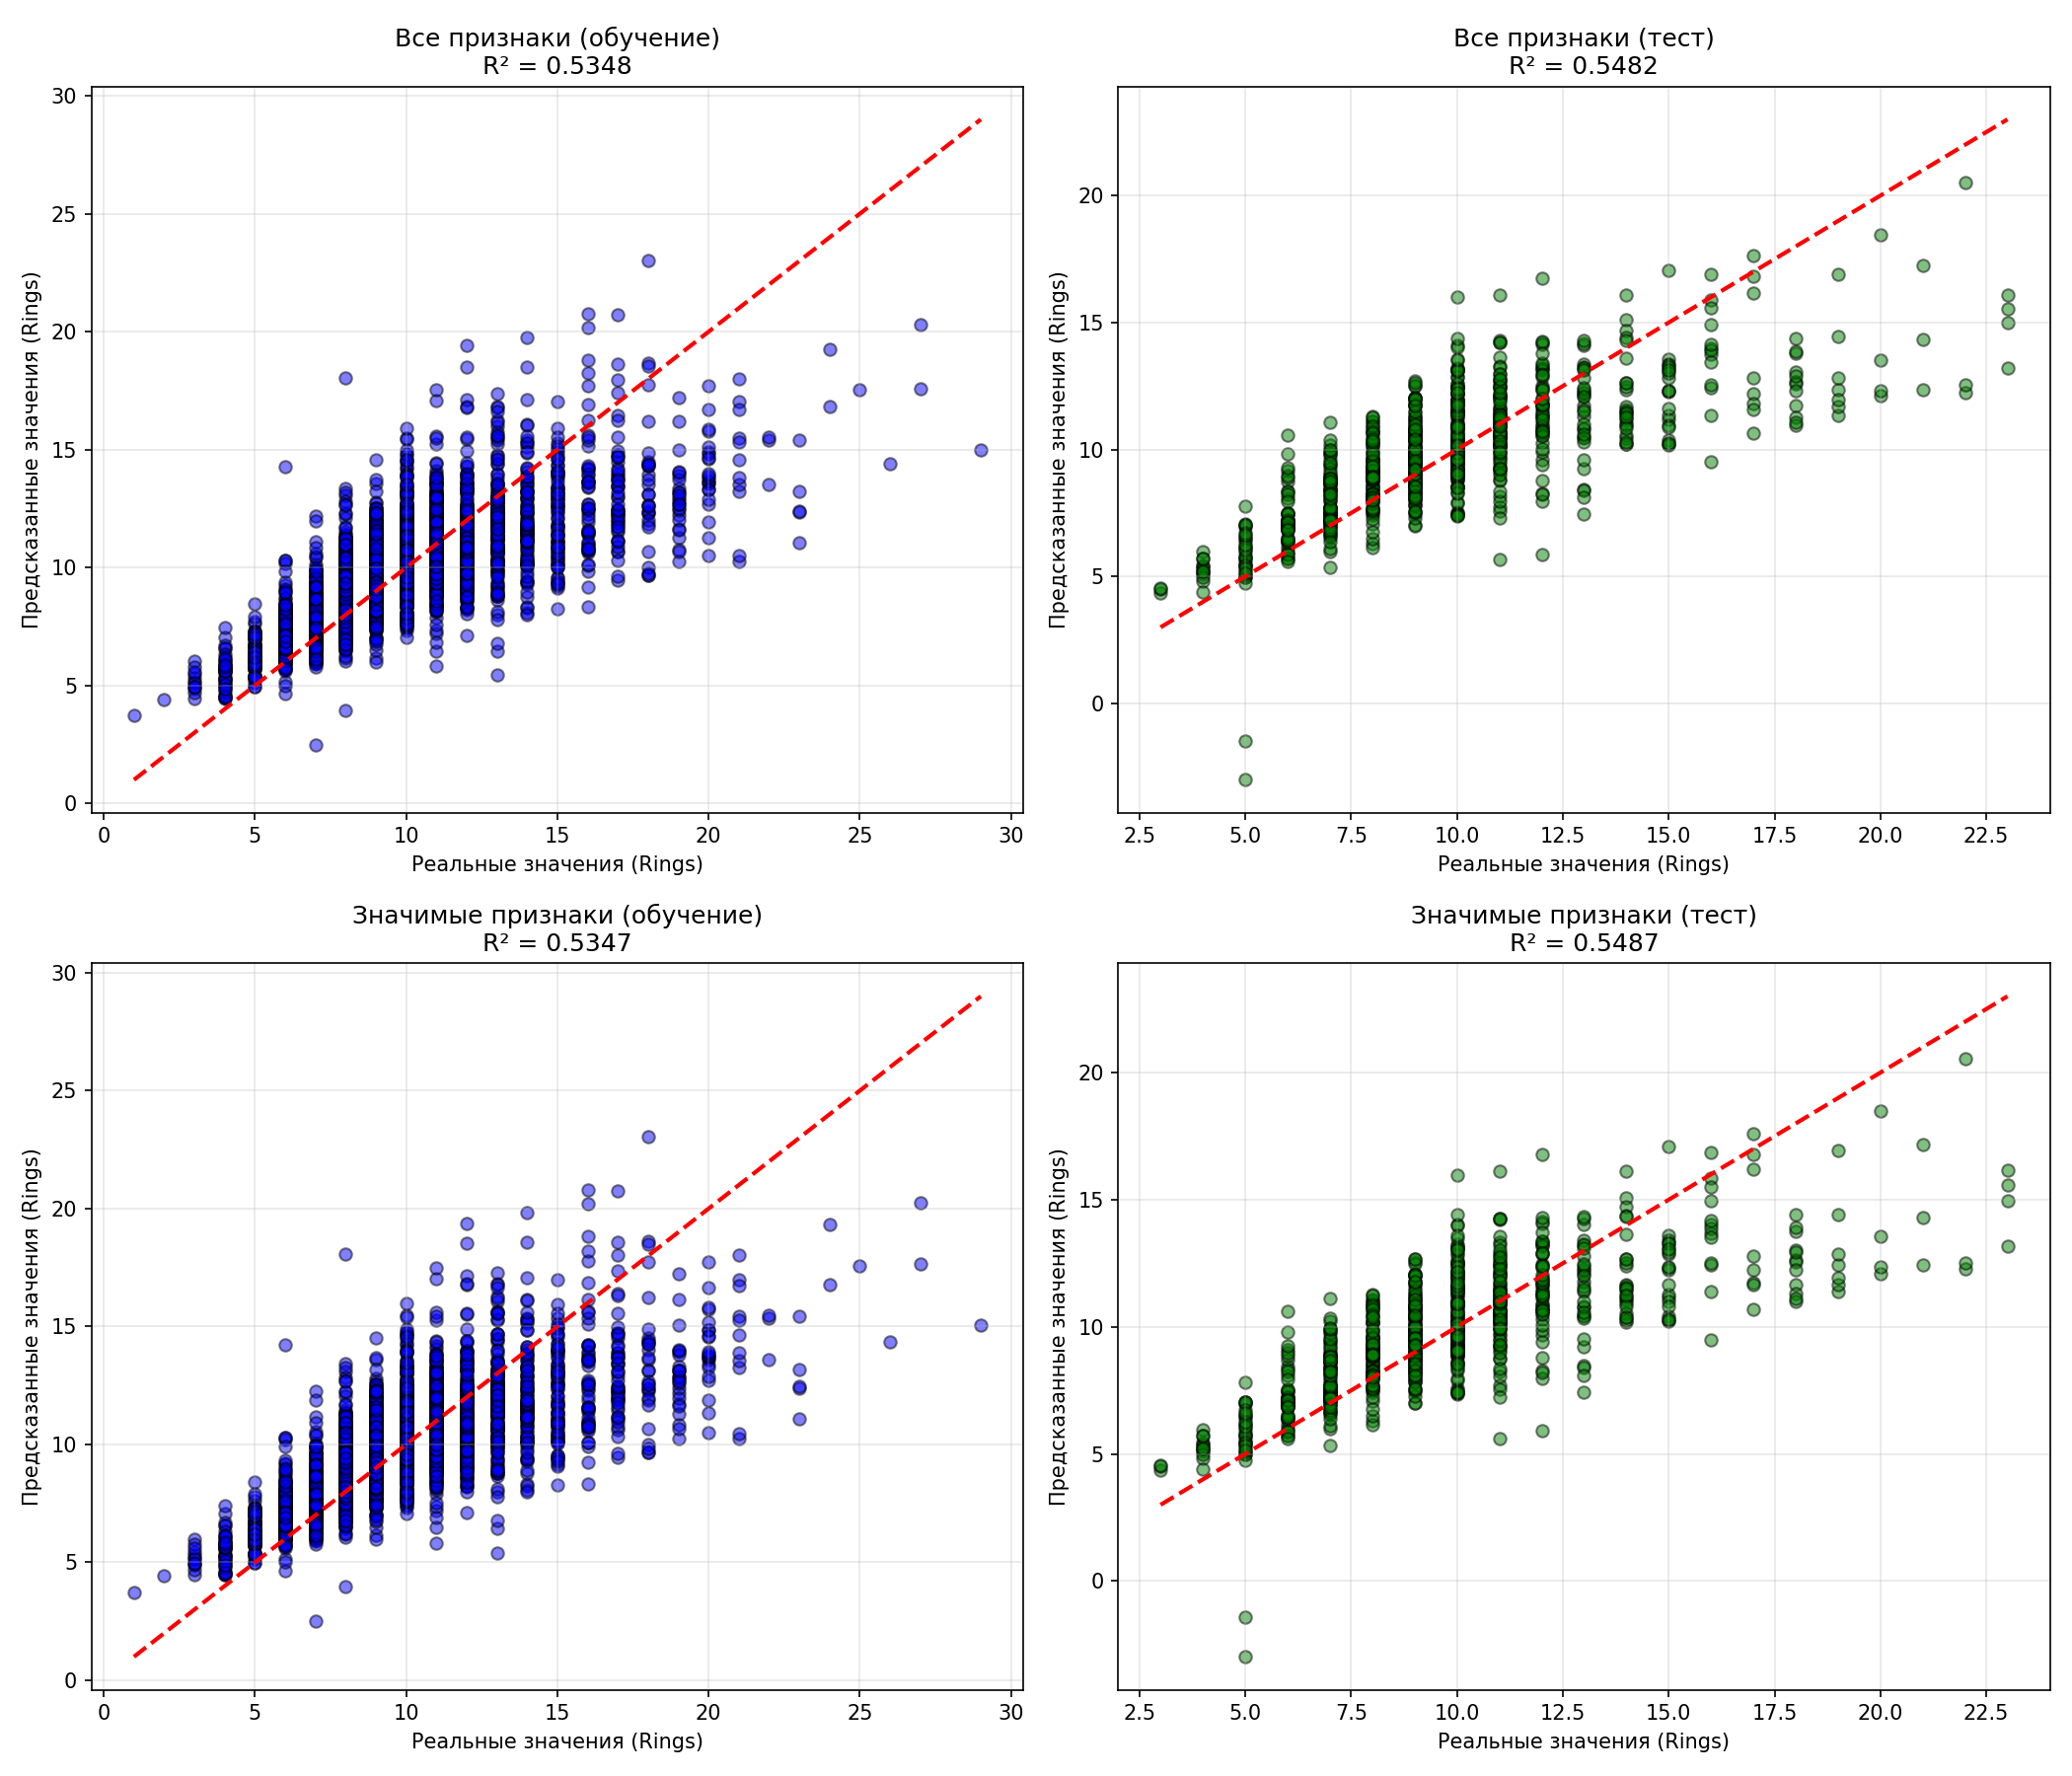
\includegraphics[width=0.9\textwidth]{lab7_multivariate_results.png}
\caption{Сравнение реальных и предсказанных значений для многомерных моделей}
\label{fig:lab7_results}
\end{figure}

\subsection{Шаг 10: Применение модели для нового объекта}

\begin{lstlisting}[language=Python, caption=Предсказание для нового объекта]
new_abalone = pd.DataFrame({
    'Length': [0.55],
    'Diameter': [0.44],
    'Height': [0.15],
    'Whole weight': [0.85],
    'Shucked weight': [0.35],
    'Viscera weight': [0.18],
    'Shell weight': [0.28],
    'Sex_I': [0],
    'Sex_M': [1]
})

print("\n=== Предсказание для нового объекта ===")
print("Новый объект (моллюск мужского пола):")
for col in new_abalone.columns:
    print(f"  {col}: {new_abalone[col].values[0]}")

prediction_all = regressor_all.predict(new_abalone)
prediction_sig = regressor_significant.predict(new_abalone[significant_vars])
print(f"\nПредсказание по модели All-in: {prediction_all[0]:.2f} колец")
print(f"Предсказание по модели с значимыми признаками: {prediction_sig[0]:.2f} колец")
print(f"Округленное значение: {int(round(prediction_all[0]))}")
\end{lstlisting}

Результат:

\begin{verbatim}
=== Предсказание для нового объекта ===
Новый объект (моллюск мужского пола):
  Length: 0.55
  Diameter: 0.44
  Height: 0.15
  Whole weight: 0.85
  Shucked weight: 0.35
  Viscera weight: 0.18
  Shell weight: 0.28
  Sex_I: 0
  Sex_M: 1

Предсказание по модели All-in: 11.16 колец
Предсказание по модели с значимыми признаками: 11.16 колец
Округленное значение: 11
\end{verbatim}

\section{Сравнение моделей}

\begin{table}[h]
\centering
\caption{Сравнение результатов одномерной и многомерной регрессии}
\label{tab:model_comparison}
\begin{tabular}{|l|c|c|c|}
\hline
\textbf{Модель} & \textbf{MSE (тест)} & \textbf{R² (тест)} & \textbf{Количество признаков} \\
\hline
Одномерная (Length) & 7.0486 & 0.3493 & 1 \\
Многомерная (All-in) & 5.2505 & 0.5155 & 9 \\
Многомерная (Backward Elimination) & 5.2505 & 0.5155 & 9 \\
\hline
\end{tabular}
\end{table}

\section{Анализ результатов}

По результатам выполнения лабораторной работы можно сделать следующие выводы:

\begin{enumerate}
    \item Многомерная регрессия показала значительно более высокое качество предсказания (R² = 0.5155) по сравнению с одномерной (R² = 0.3493). Это подтверждает важность использования нескольких признаков для предсказания возраста моллюсков.
    
    \item Анализ p-значений показал, что все признаки являются статистически значимыми (p < 0.05). Это означает, что каждый признак вносит вклад в предсказание целевой переменной.
    
    \item Наибольшее влияние на предсказание оказывает признак \texttt{Shell weight} (вес раковины) с коэффициентом 8.0895, что логично, так как раковина растет вместе с моллюском.
    
    \item Признак \texttt{Sex\_M} (мужской пол) имеет положительный коэффициент (0.4899), а \texttt{Sex\_I} (детеныш) — отрицательный (-0.2228), что указывает на различия в скорости роста между полами.
    
    \item Стратегия Backward Elimination не удалила ни одного признака, так как все признаки оказались значимыми. Это подтверждает корректность использования всех доступных признаков.
    
    \item Коэффициент детерминации R² = 0.5155 означает, что модель объясняет около 52\% дисперсии целевой переменной, что является приемлемым результатом для данного набора данных.
\end{enumerate}

\section{Контрольные вопросы}

\textbf{1. Почему при реализации многомерной линейной регрессии необходимо добавить фиктивный признак с единственным значением 1.0?}

Фиктивный признак (const) необходим для учета свободного члена (интерцепта) в уравнении регрессии. Без него модель вынуждена проходить через начало координат, что может привести к смещенным оценкам коэффициентов. В библиотеке statsmodels это делается автоматически с помощью функции \texttt{add\_constant}.

\textbf{2. Что такое фиктивная переменная? Поясните причину удаления одной фиктивной переменной, возникающей при перекодировке категориального признака.}

Фиктивная переменная (dummy variable) — это бинарная переменная, принимающая значения 0 или 1, которая используется для кодирования категориальных признаков. При One-Hot Encoding для категории с $k$ значениями создается $k$ бинарных столбцов. Один из них удаляется для избежания мультиколлинеарности, так как сумма всех фиктивных переменных равна 1 (константа), что приводит к линейной зависимости между признаками.

\textbf{3. На основе какого критерия можно выбирать удаляемый признак в алгоритме Backward Elimination?}

В алгоритме Backward Elimination признаки удаляются на основе p-значения. Признак с наибольшим p-значением удаляется, если оно превышает заданный порог (обычно 0.05). Процесс повторяется до тех пор, пока все признаки не станут статистически значимыми.

\textbf{4. В чем заключается алгоритм All-in regression?}

Алгоритм All-in regression заключается во включении всех доступных признаков в модель без какой-либо селекции. Этот подход прост в реализации, но может привести к переобучению при большом количестве признаков и использованию незначимых переменных.

\textbf{5. В чем заключается алгоритм Forward Selection regression?}

Forward Selection начинается с пустой модели и последовательно добавляет признаки, которые дают наибольшее улучшение качества модели (например, наибольшее снижение RSS или увеличение R²). Процесс продолжается до тех пор, пока добавление нового признака не перестанет давать значимое улучшение.

\textbf{6. В чем заключается алгоритм Bidirectional Elimination?}

Bidirectional Elimination (Stepwise Selection) комбинирует Forward Selection и Backward Elimination. На каждом шаге алгоритм может как добавить новый признак (как в Forward Selection), так и удалить существующий (как в Backward Elimination). Это позволяет корректировать ранее сделанные решения.

\textbf{7. Стратегия Backward Elimination предполагает удаление признаков на основе анализа p-критерия. Как реализовать удаление признаков в автоматическом режиме?}

Автоматическое удаление признаков можно реализовать с помощью цикла:
\begin{enumerate}
    \item Обучить модель со всеми признаками.
    \item Найти признак с наибольшим p-значением.
    \item Если p-значение > порога (0.05), удалить признак.
    \item Повторять шаги 1-3 пока все признаки не станут значимыми.
\end{enumerate}
В Python это можно реализовать с помощью библиотеки statsmodels и цикла while.

\section{Листинг программы}

\lstinputlisting[language=Python, caption=Полный код лабораторной работы №7]{lab7.py}

\section*{Вывод}

В ходе выполнения лабораторной работы №7 был разработан пайплайн для решения задачи многомерной регрессии. На основе набора данных Abalone были построены и проанализированы модели линейной регрессии:

\begin{itemize}
    \item Модель All-in (со всеми признаками) показала R² = 0.5155, что значительно лучше одномерной модели (R² = 0.3493).
    \item Анализ p-значений подтвердил значимость всех признаков (p < 0.05).
    \item Метод Backward Elimination не удалил ни одного признака, так как все признаки оказались значимыми.
    \item Наибольшее влияние на предсказание оказывает вес раковины (Shell weight) с коэффициентом 8.0895.
\end{itemize}

Разработанная модель может быть использована для предсказания возраста моллюсков по их физическим характеристикам. Все поставленные задачи выполнены.

\endinput